\documentclass{acm_proc_article-sp}

% UTF8 encoding and scalable fonts
\usepackage[utf8]{inputenc}
\usepackage[T1]{fontenc}

\usepackage{microtype}
\usepackage{graphicx}
\usepackage{subfigure}
\usepackage{booktabs}
\usepackage{listings}
\usepackage[hyphens]{url}
\usepackage[hidelinks]{hyperref}

% \usepackage{doi}
% \setlength{\paperheight}{11.69in}

\begin{document}

% Leave as is
\conferenceinfo{5th Seminar on Research Trends in Media Informatics (RTMI '13).}{\\February 2013, Ulm University, Ulm, Germany.}
\CopyrightYear{2013}

\title{Interaction Issues during Autonomous Driving}

\numberofauthors{1}
\author{
\alignauthor
Tamino P.S.M. Hartmann\\
       \affaddr{Institute of Media Informatics}\\
       \affaddr{Ulm University}\\
       \affaddr{Ulm, Germany}\\
       \email{tamino.hartmann@uni-ulm.de}
}

% Hyphenations here:
\hyphenation{au-to-no-mo-us}

\maketitle
\begin{abstract}
This paper represents a short overview over control hand-off issues for automated automotive applications – meaning self-driving cars.
We will shortly take a look at existing knowledge and then extrapolate problems and solutions that might be of interest.
%TODO Might want to reword that :P
Where required, we will fill knowledge gaps with careful presumptions.
\end{abstract}

\keywords{autonomous vehicle, self-driving car, driver-vehicle interaction, control hand-off}

\section{Introduction}

Autonomous vehicles have a surprisingly long history, although they have only recently become technologically feasible.
First widely proposed by Norman Bel Geddes in his book Magic Motorways \cite{geddes2009magic} and at the World Fair in 1939, driverless cars were first thought to be cars that were controlled by technology within the road.
Only in the 1980's did the steering control move from the road into the car itself.
There it has stayed for now, although due to the significant adoption of ubiquitous networking, the first systems have now been proposed where individual cars communicate with each other to further improve congestion and transport flow – effectively moving control back to a common intelligence.

While the first estimates concerning the adoption of autonomous vehicles proved to be widely optimistic, we have now come into a time where the technology is capable of fulfilling this science fiction dream.
Google's self-driving car \cite{www:google_car} has been widely reported on, although by far not the first project within the field.
First large steps were made by the introduction of the DARPA-funded Autonomous Land Vehicle project in the United States of America.

%TODO Correct ref.
Indeed the first cars with partial autonomous capabilities have entered commercial production and are publicly available, as can be seen in section \ref{current_tech}.
These capabilities include systems that keep a car traveling within its lane, park the car, and systems that react to emergency situations, for example by beginning breaking the vehicle even before the driver has had a chance to react.

As these systems continue to increase in modern cars, the role of the driver is transforming from the single controlling entity to a more copilot-like role.
However the current state of affairs hints that some interaction will always be required by the driver, for example when the autonomous drive system is confronted with a situation it cannot handle.
This is where a potential massive problem exists: the hand-off of control from the vehicle to the driver.

We will therefore in the following take a closer look at the current state of the technology, how working prototypes handle the issue, and what might be future solutions to arising problems.
Our reasoning will be based on own contributions and existing work done in automation, such as airplane and train automation, where we will study whether findings can be transferred to autonomous cars.

\subsection{Preamble}

Due to the secretory nature of automotive manufacturers, only inconclusive knowledge is accessible to the general public.
This paper is therefore based mostly on presumptions and extrapolations from published videos and articles.
As the University of Ulm has no self-driving car, research for this topic was also beyond the scope of the seminar for which this paper was written.

\subsection{Content of this Paper}

In this paper we will first give an overview over the current state of the technology to the best of our current abilities.
This will include a section on autonomous technology in non-automotive fields, labeled as off-domain, and a section on existing and available technology already deployed in purchasable cars.

We will then come to the main topic of this paper and provide a discussion of the hand-off problem and possible solutions.
Finally, we will conclude the paper with an overview and ideas for future research.

\section{Current Technological State}

In this section we will take a look at existing work on the topic of interaction issues between autonomous vehicles and their operators.
We will begin by shortly locking at alternative fields where automation is already actively in use, mainly aircraft and trains, henceforth labeled as off-domain automation.
Then we will give a brief topic-specific general overview of existing technology and solutions in the automotive field by functionality, from single systems up to comprehensive fully automated vehicles.

\subsection{Existing Research}

Little research work in the form of public papers exists at the time of writing.
We believe this to be because of two reasons: the relatively young age of the technology and the commercial secrecy of vehicle manufactures.

An article in the Huffington Post \cite{www:huffington_post} brought the work of Clifford Nass to our attention who has begun working on interaction issues.
However no published work has yet been publicly been made available.

A draft also exists that parallels the proposed paper, but to our knowledge has not been finished yet \cite{cummings:authority}.
It will also be incorporated into the proposed paper, especially as it has a similar approach to the topic.
The draft is however not fully fledged out yet, and thus only of specific use.

The point of commercial secrecy is a harder hurdle in the context of writing this paper however.
Some research showed that a multitude of marketing videos and articles exist that show the various features that have been developed and integrated into existing cars.
However, these publications concentrate mainly on selling the technology, and are therefore not very informative from a technical view and biased as they hide advantages and difficulties.

\subsection{Current Technology}
\label{current_tech}

Although most companies that have begun developing autonomous car technology remain relatively secretive, some information is publicly available.
Therefore we will take a look at some systems of interest that are known to exist at this time, including the few systems already commercially available.
We will briefly highlight their technological standing and what can be deduced for interaction issues from how they have implemented the technology.
We will begin by taking a look at off-domain work done for automation, as some of our later points will be based on these.

\subsubsection{Off-Domain}
% Note that trains haven't been considered in the related work yet, might want to concentrate more on them instead of airplanes.
% Aircraft, boats, trains, spacecraft!

Automation for vehicles is not constrained only to the car.
Airplanes have routinely been flying with the so-called autopilot since its widespread adoption around the 1950's.
In 1947 a military aircraft made a transatlantic flight completely on autopilot, including landing and starting, for the first time.
Since then the usage of autopilots in commercial and military aircraft has become part of our everyday lives.
Notably, autopilots were developed to decrease the need of constant vigilance by pilots on long flights.

A more simple use-case can be found in self-steering gear for ships.
Here too the human operators of the ships face long monotone traveling where little input is required but constant vigilance.
The self-steering gear allows the operators to transfer the task of keeping the ship on course to a mechanical automation, allowing them to relax.

In the locomotive area, fully autonomous train systems already exist.
However, it is important to note that this is mainly due to the fact that unlike airplanes and ships, trains run on predefined given routes.
Also helpful for the automation of trains is that from the start, strong coordination was required to keep trains from running into each other, as they have no capability to avoid a collision by moving out of the way.
Generally speaking, autonomous systems for trains make strong usage of the comprehensive right-of-way systems already in place.

%TODO operators who have not undergone comparable training --> pick that up later!
Taking a closer look at the capabilities of these systems allows us to grant some insights into the requirements of automotive automation.
From a human resource point of view, pilots, helmsmen, and engineers are for the most part highly trained specialists.
Most of the cars on the road nowadays are driven by operators who have not undergone comparable training.
From a more technological view, cars pose a unique challenge.
A right-of-way systems exists, however it is not as static as for trains but a highly dynamic system.
Furthermore, because cars operate mainly in highly populated areas, a multitude of factors need to be considered for navigation and collision avoidance.
Just the number of freely moving vehicles increases the difficulty of successive automation by a large margin.
Add to that that cars share their operational space with people, bicyclists, trucks, and more, and you receive an environment not really suited for automation.
Concerning their operational environment another point needs to be considered; the fact that the road system on which cars travel is extremely extensive, with a wide range of conditions that need to be considered.

Another problem can be found in the spontaneous operation; unlike trains, and to some extent airplanes, no schedule exists that coordinates their travels.
Given human nature, this also seems nonviable to implement, as humans would generally consider these limiting factors.
This can be found in the social and cultural believe that owning a car is considered to be the ultimate freedom, as it allows one to travel when and where one wants.

Compared to the above three fields, cars also have a few advantages.
For one, their response time can be significantly faster due to high acceleration and deceleration values.
Inertia and vehicle size are also significantly more manageable than say, trains or ships.
As cars operate on ground level in a very open environment, they are also capable of avoiding obstacles much better than trains, possibly simply by safely moving off the road to avoid an impending collision.
The market diversity of automobile manufacturing is also higher than in other vehicle fields.
As can be seen today, a multitude of companies are already developing independent systems.
That would decrease the risk of a single point of failure, increasing the safety of traffic in general.

\subsubsection{Singular Systems}

In this section, we will take a look at systems that handle single aspects of driving for the driver.
These include for example systems for automatic parking, lane assistants, or collision avoidance systems.
An overview of interaction solutions that are used by these is given at the end of this section, as these will be relevant for hand-off considerations later.

An interesting system is the Distronic system from Mercedes Benz \cite{www:mercedes_pre_safe}.
This system is in essence an adaptive cruise control that is aware of vehicles in front of the car.
The information on vehicles in front of the car is captured via three radar systems; two short range that also cover adjacent lanes and a single long range radar for vehicles further away in the same lane.
Normally, this system automatically adjusts the speed of the cruise control to remain within the flow of traffic, as given by the vehicle in front.
However, should the vehicle in front suddenly break, the system can also initiate a full breaking maneuver.
During these tasks, it continuously gives the driver feedback to what is happening.
This also includes a gauge that tells the driver how far the vehicle in front is away.
Notably, the system waits as long as possible before intervening in emergency situations, allowing the driver to take over control.
If a collision is imminent however, the system will slow the car whether or not the driver breaks.
Such systems are already available from a multitude of companies; see also the similar system from Toyota here \cite{www:toyota_pcs}.

Such fully adaptive cruise control allows drivers to let the car handle long voyages on highways or even the stop-and-go of a congested road.
Notably however, the system will not move the car from a standstill, as current law prohibits a car to start moving on its own.
It also does not handle steering, although land assist systems exist that can cooperate with such an adaptive cruise control.
Driver interaction is however always required, and the responsibility remains with him too.

Lane assist, such as the system developed by Volkswagen \cite{www:vw_lane_assist} is a system that keeps a car oriented within a lane, for example when driving on the highway.
The system by Volkswagen works upwards of 65km/h.
It detects the lane markings via a camera mounted on the rear mirror and adjusts the steering of the vehicle by itself, within certain bounds.
If the correction necessary lies outside the limits, the steering wheel vibrates to signal the driver that he has to control the steering.
If the system detects that the driver has taken his hands from the steering wheel, it gives warning and automatically deactivates after a set time.

Automation is also available for specific tasks, such as parking a car.
Toyota has developed and produced the Intelligent Park Assist system \cite{www:toyota_i_park_assist}.
This system can measure a parking slot while driving by and then control the steering.
Notably, control of the speed remains with the driver; it is up to him to break when the park location has been reached.
A video presentation of the system can be found here \cite{www:toyota_ipa_video}.

Apart from handling the steering of parking, systems have long been in development for parking a car remotely and or completely by itself.
Most systems nowadays still require the driver to stand nearby and oversee the maneuver, but systems that would in effect eliminate the need for valets and allow the car to truly park itself and later on pick its driver up again have also been in development for a while now.

Another such system that we will take a look at is the Attention Assist system from Mercedes Benz \cite{www:mercedes_attention_assist}.
Here, the car company has developed a system that can detect when a driver is fatigued and alert him to take a break.
While primarily not an automation system, it has a range of implications for autonomous driving.
As long as a driver will still be required to be present and available to control the car, a system must be in place that can control for these variables.
The Attention Assist presents a possible system that might be incorporated into a suite of sensors for monitoring the driver.
More on this topic can be found in section \ref{solutions}.

In general one notices that all of the systems have been produced and are publicly available require the driver to be actively in control at all times – either by keeping his hands on the control mechanisms of the vehicle or by being physically near it.
This is due to the current legislation which enforces that a human driver must always be there to take over and who is responsible for the safety of the vehicle.
The next logical step then is to take the driver out of the loop and to combine all these systems into a fully autonomous vehicle, as seen in the next section.

\subsubsection{Comprehensive Systems}

Here, we take a look at the limited knowledge available on the continuous development of fully autonomous cars.
Mainly we will concentrate on the work done by Google, due to their comparatively high yield of information compared to other companies.

\begin{figure}
	\centering
	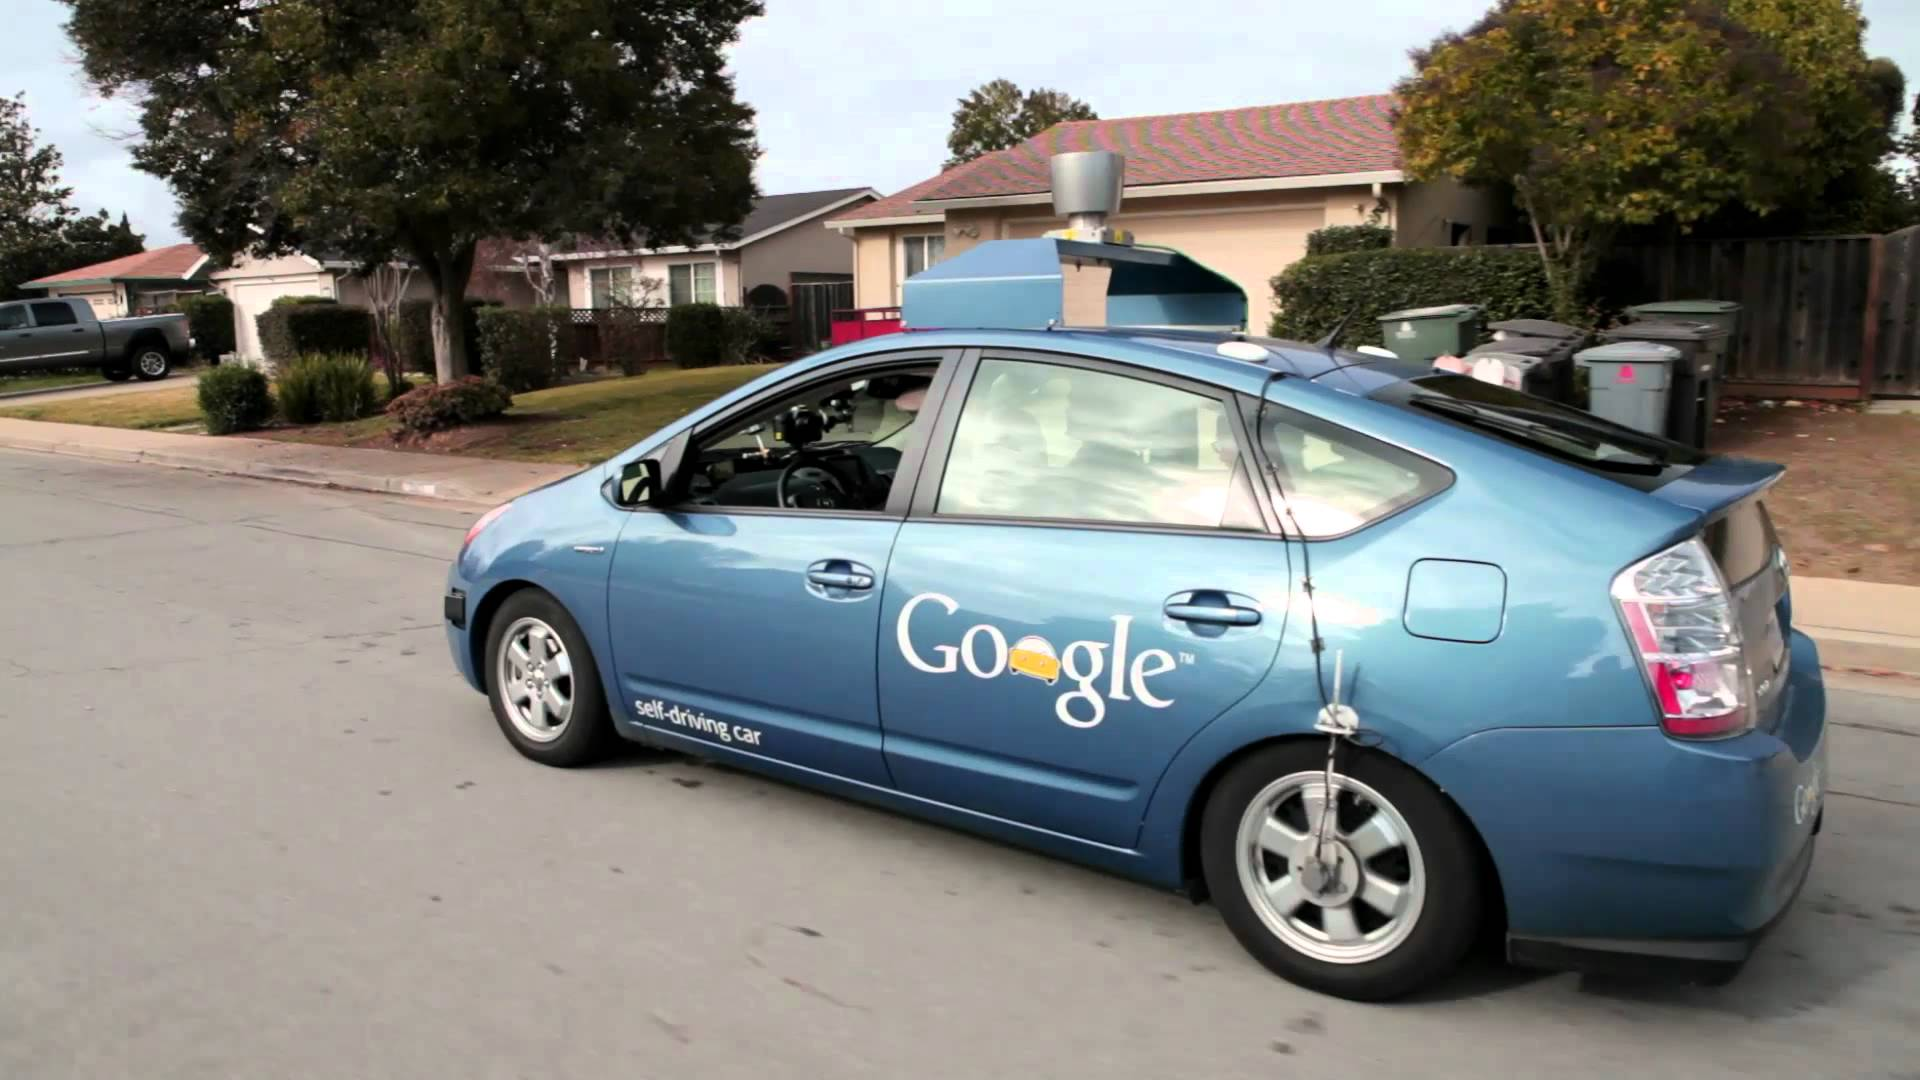
\includegraphics[width=\columnwidth]{img/google_vehicle.jpg}
	\caption[Google Self Driving Car]{An image of one of Google's self driving cars.}
	\label{fig:google_vehicle}
\end{figure}

Figure \ref{fig:google_vehicle} shows one of Google's fully autonomous vehicles.
To note is the LIDAR\footnote{LIDAR: LIght raDAR system.} sensor on the roof and the odometer visible on the back wheel.
Google has a fleet of vehicles – a dozen on the road at any given time – and has driven almost 500,000 kilometers with them in total \cite{www:google_blog_miles}.

\begin{figure}
	\centering
	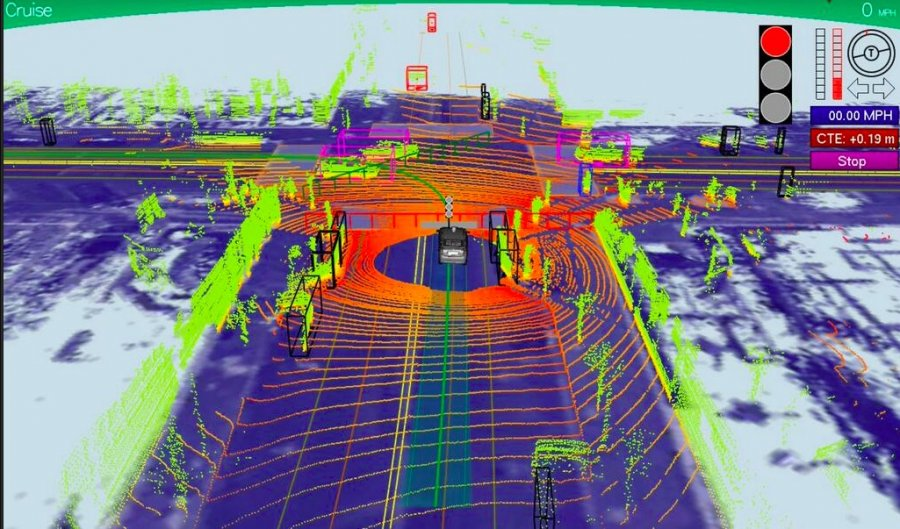
\includegraphics[width=\columnwidth]{img/google_tech_view.jpg}
	\caption[Tech View]{A screenshot of the digital representation shown to the vehicles' occupants for debugging purposes.}
	\label{fig:google_tech_view}
\end{figure}

The vehicle takes in its surroundings with a range of sensors and creates a digital representation of its surroundings.
This representation includes information of pedestrians and other vehicles, moving obstacles, the surroundings, information on the road, and the course that the vehicle plans on taking.
This digital representation is also available for the developers in the vehicle via a large screen that renders it, updating in real-time as the vehicle drives.
While primarily meant for debugging purposes, one journalist noted that such a view would alone already be nice to have in any modern vehicle, as there are no blind spots and it gives a nice overview of the road situation.
Figure \ref{fig:google_tech_view} shows a screenshot of the display.

Google's self driving car is currently only capable of driving under almost ideal situations.
If the car encounters a construction cite for example, it gives an auditory warning that the driver will have to take over control within the next mile, for example \cite{www:newyorker_google_car}.
The above citation is the only mention we found of how Google's vehicles handle the hand-off.
Of course, given advanced warning only works if the vehicle has a chance of detecting the imminent hand-off early enough to give the driver ample time to adjust and take over control from the automation.
Ideally of course, the vehicle would never have to hand control to its driver – but the technology is still a good bit away from that level of intelligence.
One must always keep in mind that computers have difficulties handling a task in an open system, such as driving a vehicle through a highly variable environment.

Google is not the only company working on developing self driving cars.
Mercedes-Benz also has a prototype in the works which has already successfully driven some distance \cite{www:mercedes_autonomous}.
From the video it is however clear that the car navigates on a predefined and mapped route that has been prepared for it.
To our knowledge, Google's cars do not require prepared courses.
However unlike Google, the vehicle uses only standard sensors commonly available – the LIDAR system is currently still relatively expensive and thus unsuited for mass production.
We have no knowledge on how the vehicle from Mercedes-Benz handles hand-off.

\section{Current and Future Issues}
%Continue here

This section explains the issues that already exist and issues that might and or will arise due to autonomous vehicles to the best of our abilities.

\subsection{General Assumptions}
%reword

Here we will briefly highlight what assumptions we make concerning autonomous vehicles.
This includes for example that the system will never actively cause an accident (due to fail-safe behavior).
We will also define the role we assume the driver to have and how he will fulfill it.
This should be done to allow us to focus only on the interaction aspects and not on the general technological hurdles that need to be overcome.

\subsection{Driver Readiness and Capabilities}
% psychological issues

A major issue is the attention span of drivers.
It has been shown that humans tend to lose focus when supervising an autonomous system that seldom requires interaction.
Therefore measuring the driver alertness and adapting how and if the car hands control over to the driver based on it should be considered also.

An increase in automation also implies that drivers will miss out in experience with road situations that are nowadays still common.
Mainly this means that drivers will become increasingly less capable of reacting correctly in the event that the autonomous system requires their assistance, even if they have been notified to the best of the systems capabilities beforehand.

This will also lead us to look at how to best convey required situational awareness to a driver in a possibly time-critical situation.
That again ties in with using attention assistance systems to monitor what information the driver requires to react best.

An important point to remember when considering autonomous systems independent of the vehicle they control however is the capabilities of their human counterparts.
Pilots and train engineers are for the most part highly trained.
Chauffeurs for cars come near to the concept, but autonomous cars will in general be used by the general population.
A population that has a varied range of experience, physical handicaps, and for whom driving is a tool to use instead of a profession.

Also mention the article (if you can find it) where that one journalist said that just the display of what the car senses would be an enormous help for driving.
Could imply that the hand-off might not be such a huge problem if the driver has such information and can react on it.
Hell, the car could even highlight the problems etc. well before they become critical.

\subsection{Control Hand-off Issues}
\label{hand_off_issue}
%TODO This is actually the main topic, move up and display more prominently

Even when the hand-off is successful (implying that the driver is in full control of the vehicle and aware of the fact), he will take a moment to understand the situation – moments he might not have.
It is even possible that due to the high automation, drivers become unfamiliar with driving, lowering their capabilities to react in a timely and correct fashion to an emergency.
This could actually increase the risk of an accident happening.

\begin{quote}
The most dangerous moment in a self-driving car involves no immediate or obvious peril.
It is not when, say, the computer must avoid a vehicle swerving into its lane or navigate some other recognizable hazard of the road -- a patch of ice, or a clueless pedestrian stepping into traffic.
It is when something much more routine takes place: The computer hands over control of the vehicle to a human being.
In that instant, the human must quickly rouse herself from whatever else she might have been doing while the computer handled the car and focus her attention on the road.
As scientists now studying this moment have come to realize, the hand-off is laden with risks.
\end{quote}
From \cite{www:huffington_post}.

% Not sure if the quotes can be used thus, but keep for now...
\begin{quote}
This brings up the most challenging obstacle on our road to the autonomous- driving future: managing the handoff.
For as long as anyone, even Google, is willing to predict, cars will by necessity be semiautonomous; human drivers will still have to play some role.
But figuring out what that role will be is complicated.
Are we pilots or copilots? How far out of the loop can we be taken?
\end{quote}
From \cite{www:wired}.

Here we will take a look at the most important interaction issue – the hand-off of control from the vehicle to the driver.
The two quotes are an excellent starting point for any of our work.
This will include a comparison of how it is done in current technology and how it will evolve as self-driving cars become better and driver assistance is required less frequently.
We will also consider limiting factors such as when the driver cannot be trusted to be fully capable of controlling the vehicle and whether the system should evaluate if it has a better chance of avoiding problems by not initiating a hand-off in the first place.

\section{Solutions}
\label{solutions}
%TODO come up with some novel solutions that might actually be feasibel – also consider changing the way drivers are trained! Also add in psychological things to consider, such as the switch found in trains to check if the driver is still alert

In this section we will discuss proposed solutions to the aforementioned issues, if available.
We will also offer up our own solutions based on existing work and technologies.
This section will most likely be highly speculative and thus will have no existing work to be based on.

A solution to the problem of drivers not being able to safely take control from the automation could be the adaption of how drivers are trained.
Apart from the basics of driving a car, courses on how to react in emergency situations could become necessary.
Always remaining ready is however not a task that many humans can easily do – however they will still need to drive.
To solve this, we propose a system for labeling automation systems in respect to driver capabilities.
Fully autonomous vehicles that would always drive so that no driver interaction is required would be free to use for everyone.
These might however be limited in where they drive and how fast they drive.
This would serve to allow the automation to drive in a safe environment that has the least amount of distractions possible, effectively rendering the need for a manual override to zero.
On the other side of the spectrum would be cars that can act fully autonomous when the computers deem it safe, but allow or even require the driver to take over when the situation warrants it.
This might be required when crossing into a new country where the laws governing driving are substantially different, rendering the automation incapable of functioning safely.

\section{Possible Future Work}
%TODO Might want to point to the work being done by the other papers and work that should be done; alternatively, issues that MUST be solved for the technology to be safe

Here we will offer a future outlook and where further work needs to be done.
This includes systems where control of the vehicle is per default not with the driver – implying autonomous vehicles beyond their adoptive period where control is still with the driver.

\section{Conclusion}

This section will be a summary of our findings.

% do not change the bibliography style
\bibliographystyle{abbrv}
\bibliography{sources}  

\balancecolumns

\end{document}
